\documentclass[12pt,letterpaper]{article}
\usepackage[margin=1in]{geometry}
\usepackage{fancyhdr}
\usepackage[utf8]{inputenc}
\usepackage{palatino}
\usepackage{microtype}
\usepackage{hyperref}
\usepackage{graphicx}
\usepackage[hang,bf,small]{caption}
\usepackage{amsmath,amssymb,amsthm}

\setlength{\parindent}{0cm}
\setlength{\parskip}{1em}

\hypersetup{colorlinks,
	linkcolor = black,
	citecolor = black,
	urlcolor  = black}
\urlstyle{same}

\begin{document}

\begin{titlepage}
	\vspace*{4cm}
	\begin{flushright}
	{\huge
		Cattlestar Balactica \\ [1cm]
	}
	{\large
		ENGR 421 -- Individual Lab Report \\ [3cm]
	}
	\end{flushright}

	\begin{flushright}
	18 April 2013 \\
	Soo-Hyun Yoo
	\end{flushright}

\end{titlepage}

\newpage

\section*{Done}

\subsection*{Website}

I have set up the team's website as a WordPress installation on a personal
server, shown below.

\begin{figure}[!h]
	\centering
	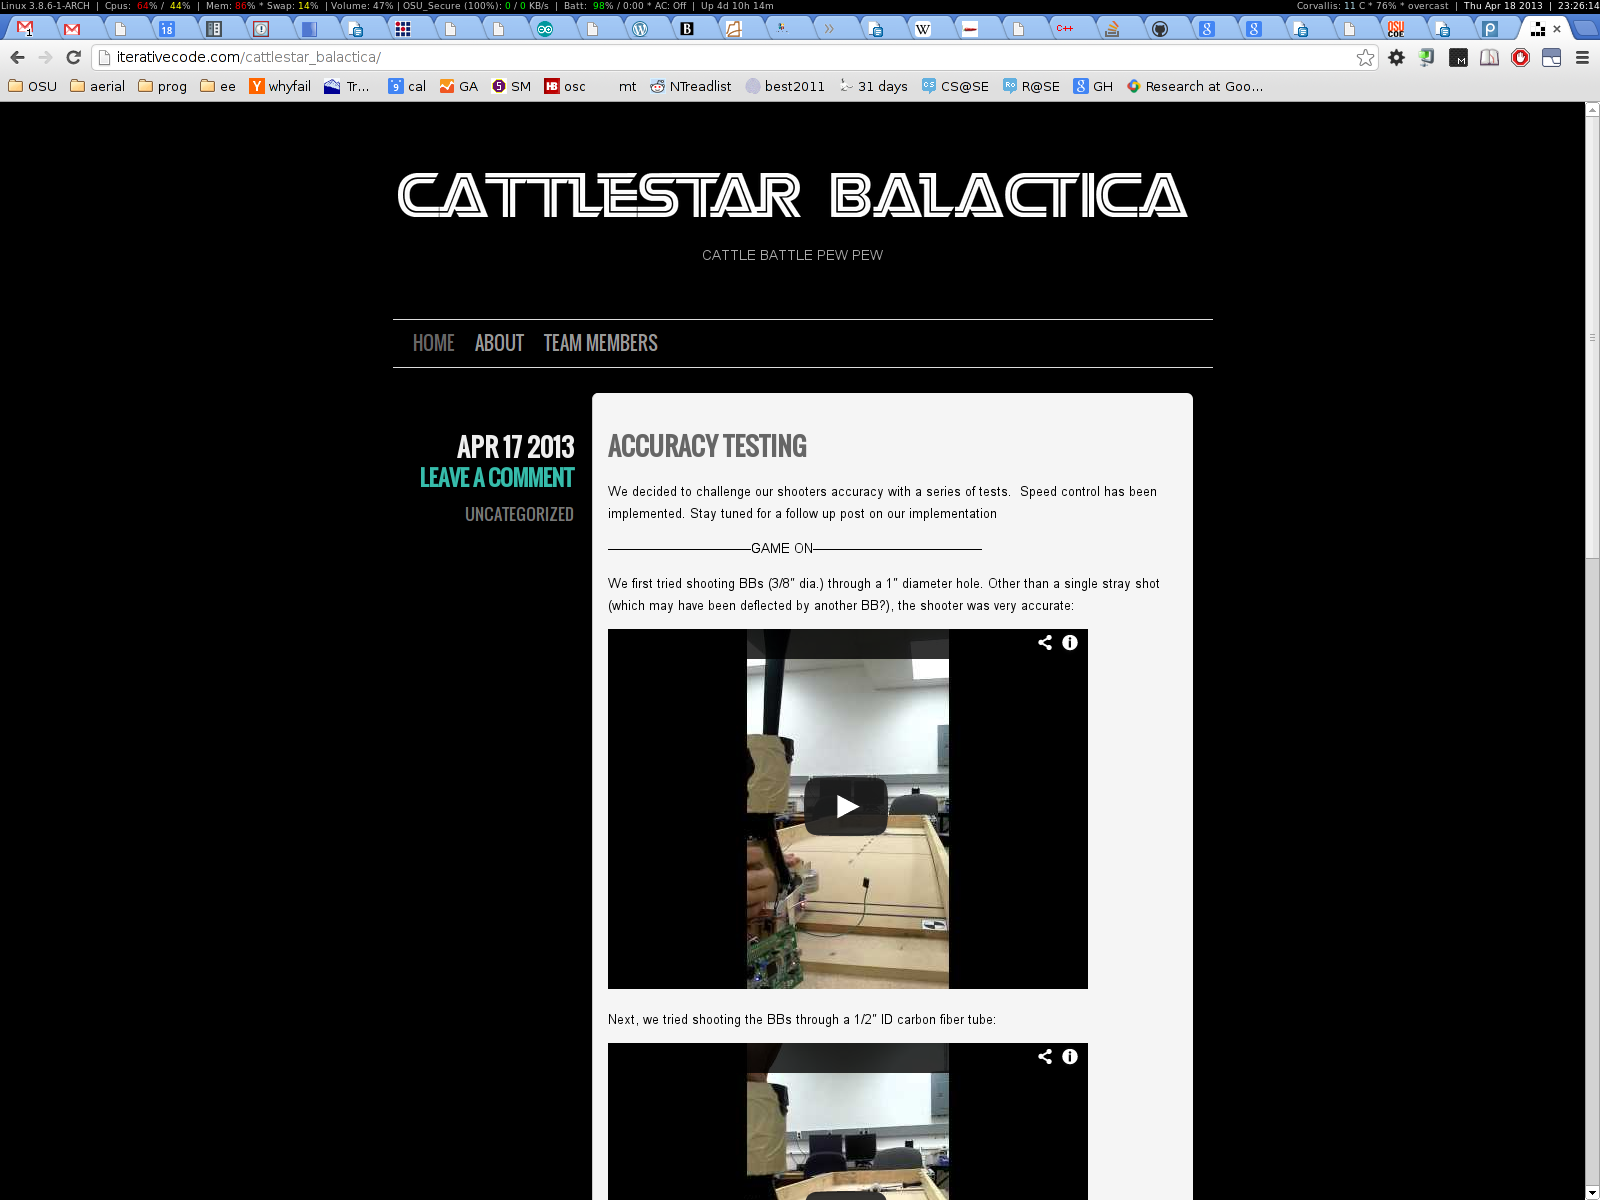
\includegraphics[width=0.6\textwidth]{website.png}
	\caption{Website set up on iterativecode.com/cattlestar\_balactica.}
	\label{fig:website}
\end{figure}


\subsection*{BB Velocity Control}

In addition to running the shooter off the STM32F4 Discovery Board instead of
an Arduino, I have set up a magnetic rotary encoder to provide the
microcontroller with rotational velocity feedback for simple velocity control
of the BBs. Using the photogate velocimeter in the lab, the actual velocity of
the BBs was confirmed to be consistent.


\subsection*{OpenCV Filtering and Edge Detection}

Basic color filtering and edge detection were implemented with OpenCV. The
results are shown below.

\begin{figure}[!h]
	\centering
	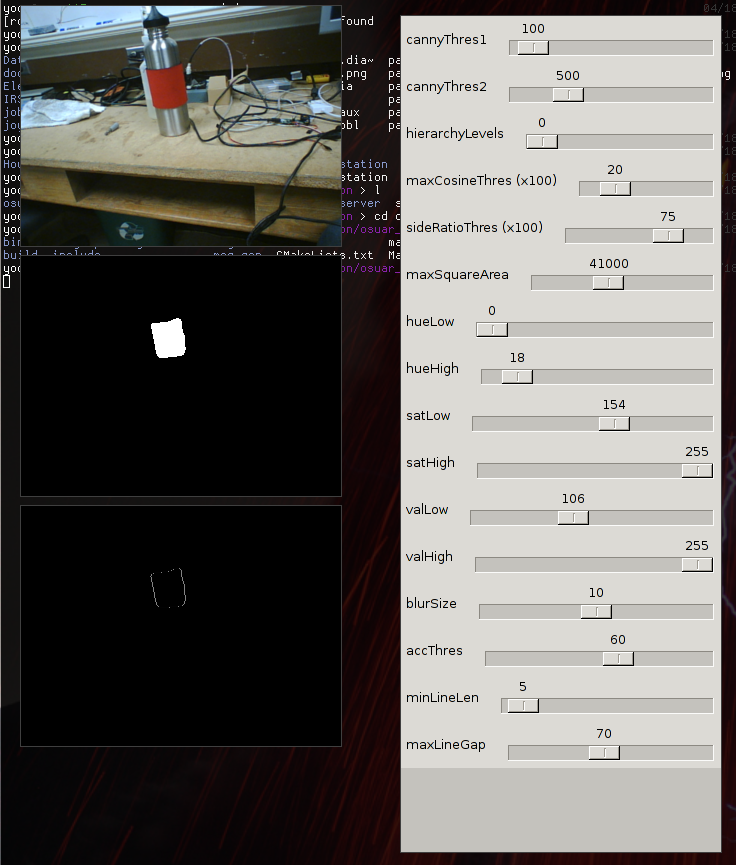
\includegraphics[width=0.6\textwidth]{vision.png}
	\caption{Basic color filtering and edge detection. Here, the thresholds are
	set to detect bright red.}
	\label{fig:vision}
\end{figure}


\subsection*{Magnetic BB Deflection}

With the BB velocity under control, I further tested the magnetic BB deflection
system and found that due to the shooter having only one wall (instead of two
to squeeze the BB into the same tight trajectory -- it is a prototype, after
all), I could not conclusively test the consistency of the deflection system.
The 3D model of the shooter is being finished and will be 3D printed by early
next week.

\section*{Todo}

In the coming week, I will use the fiduciary markers on the playing field to
rectify the board and locate pucks regardless of camera placement as long as
all four markers are visible.

I will also start working on code for controlling the linear rail.

\end{document}

